\onehalfspacing
\section{Đề số 10}
\graphicspath{{./img/}}
\begin{bt} 
	Tính giá trị của biểu thức
	\begin{enumerate}[a.]
		\item $A=\frac{4^5 \cdot 9^4-2 \cdot 6^9}{2^{10} \cdot 3^8+6^8 \cdot 20}$
		\item $\mathrm{B}=1+3+3^2+3^3+\ldots+3^{2015}-\frac{3^{2016}}{2}$
	\end{enumerate}
	\loigiai{
		\begin{enumerate}
			\item A=$\frac{2^{10} \cdot 3^8-2^{10} \cdot 3^9}{2^{10} \cdot 3^8+2^{10} \cdot 3^8 \cdot 5}=\frac{2^{10} \cdot 3^8(1-3)}{2^{10} \cdot 3^8(1+5)}=-\frac{1}{3}$
			\item Đặt $M=1+3+3^2+\ldots+3^{2015}$\\
			Ta có $3 \mathrm{M}=3+3^2+3^3+\ldots+3^{2016}$\\ $3 \mathrm{M}-\mathrm{M}=3^{2016}-1 \Rightarrow \mathrm{M}=\frac{3^{2016}}{2}-\frac{1}{2}$\\
			Khi đó $\mathrm{B}=\frac{3^{2016}}{2}-\frac{1}{2}-\frac{3^{2016}}{2}=-\frac{1}{2}$\\
		\end{enumerate}
	} 
\end{bt}

\begin{bt}
	\hfill
	\begin{enumerate}[a.]
		\item Tìm $x$ biết: $\frac{15}{28}-\left|x-\frac{3}{14}\right|=-\frac{5}{12}$
		\item Tìm $x$, y nguyên biết: $25-y^2=4(x-2016)^2$
	\end{enumerate}
	\loigiai{
		\begin{enumerate}
			\item $\left|x-\frac{3}{14}\right|=\frac{15}{28}+\frac{5}{12} \Leftrightarrow\left|x-\frac{3}{14}\right|=\frac{80}{84}$\\
			$
			x-\frac{3}{14}=\frac{80}{84} \text { hoặc } x-\frac{3}{14}=-\frac{80}{84} \\
			x=\frac{3}{14}+\frac{80}{84} x=\frac{3}{14}-\frac{80}{84} \\
			x=\frac{7}{6} x=\frac{31}{42}
			$\\
			$\text { Vậy } x=\frac{7}{6} ; \quad x=\frac{31}{42}$
			\item Ta có $4(x-2016)^2 \geq 0$ với mọi $x$ nên $25-y^2 \geq 0 \Rightarrow y^2 \leq 25$\\
			Mà $4(x-2016)^2$ là số chính phương chẵn $\Rightarrow 25-y^2$ chẵn\\
			$\Rightarrow \mathrm{y}$ lẻ.\\
			$\mathrm{y}^2$ là số chính phương lẻ, $\mathrm{y}^2 \leq 25 \Rightarrow \mathrm{y}^2 \in\{1 ; 9 ; 25\}$\\
			+ Nếu $y^2=25 \Rightarrow 4(x-2016)^2=0 \Rightarrow x=2016$\\
			+ Nếu $y^2=9 \Rightarrow 4(x-2016)^2=16 \Rightarrow x=2016$\\
			$\Rightarrow(x-2016)^2=4$\\
			$x-2016=2$ hoặc $x-2016=-2$\\
			$x=2018$ hoặc $x=2014$\\
			+ Nếu $y^2=1 \Rightarrow 4(x-2016)^2=24$ không phải là số chính phương (loại )\\
			Vậy với $y= \pm 3$ thì $x=2018 ; x=2014$\\
			Với $y= \pm 5$ thì $x=2016$.\\
		\end{enumerate}
	} 
\end{bt}

\begin{bt}
	\hfill
	\begin{enumerate}[a.]
		\item Cho đa thức: $f(x)=a x^2+b x+c$.
		Biết $13 \mathrm{a}+\mathrm{b}+2 \mathrm{c}=0$.\\
		Chứng minh $\mathrm{f}(-2) \cdot \mathrm{f}(3) \leq 0$
		\item Cho các số thực $x, y, z \neq 0$ thỏa mãn: $\frac{x y}{x+y}=\frac{y z}{y+z}=\frac{x z}{x+z}$\\
		Tính giá trị cuả biểu thức: $\mathrm{M}=\frac{\mathrm{x}^2+\mathrm{y}^2+\mathrm{z}^2}{\mathrm{xy}+\mathrm{yz}+\mathrm{xz}}$.
	\end{enumerate}
	\loigiai{
		\begin{enumerate}
			\item Ta có $f(3)=9 a+3 b+c$ ; $f(-2)=4 a-2 b+c$ \\
			$f(3)+f(-2)=13 a+b+2 c=0$ => $f(3)=-f(-2)$ \\
			$\Rightarrow f(3) \cdot f(-2)=-f(3)^2 \leq 0$
			\item Vì $\mathrm{x}, \mathrm{y}, \mathrm{z} \neq 0$ nên theo bài ra ta có: \\
			$\frac{x+y}{x \cdot y}=\frac{y+z}{y \cdot z}=\frac{x+z}{x \cdot z}$ \\
			$\Rightarrow \frac{1}{x}=\frac{1}{y}=\frac{1}{z} \\
			\Rightarrow \mathrm{x}=\mathrm{y}=\mathrm{z}$.\\
			Thay $\mathrm{x}=\mathrm{y}=\mathrm{z}$ vào $\mathrm{M}$ ta được $\mathrm{M}=1$.
		\end{enumerate}
	} 
\end{bt}

\begin{bt}
	Cho tam giác $\mathrm{ABC}$ vuông ở $\mathrm{A}$, có phân giác $\mathrm{BD}, \mathrm{CE}$ cắt nhau ở $\mathrm{I}$. Gọi $\mathrm{M}, \mathrm{N}$ lân lượt là hình chiếu của $D, E$ trên $B C$
	\begin{enumerate}[a.]
		\item Chứng minh tam giác $\mathrm{ABM}$ cân.
		\item Chứng minh $\mathrm{MN}=\mathrm{AB}+\mathrm{AC}-\mathrm{BC}$
		\item Tính góc MAN.
		\item Gọi $G, K$ lân lượt là giao điểm của $B D$ và $A N ; C E$ và $A M$. Tia $A I$ cắt $G K$ ở $H$. Tính góc AHG.
	\end{enumerate}
	\loigiai{
		$$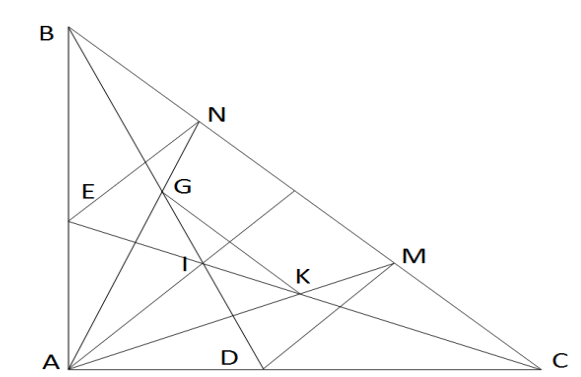
\includegraphics[width=0.55\textwidth]{10-4-lg.png}$$
		\begin{enumerate}
			\item $\triangle A B D=\triangle M B D($ cạnh huyền - góc nhọn $)\\
			=>\mathrm{AB}=\mathrm{AM}=>\triangle A M B$ cân ở B.
			\item Ta có $\triangle A E C=\triangle N E C=>\mathrm{CN}=\mathrm{CA} \\
			\mathrm{Khi} \text { đó } \mathrm{AB}+\mathrm{AC}=\mathrm{BM}+\mathrm{CN}=\mathrm{BM}+\mathrm{MC}+\mathrm{MN}=\mathrm{BC}+\mathrm{MN}
			\\ \quad \Rightarrow \mathrm{MN}=\mathrm{AB}+\mathrm{AC}-\mathrm{BC}$
			\item Từ $\triangle A M B$ cân ở $\mathrm{M} \Rightarrow A M B=\frac{180^{\circ}-A B C}{2}=90^{\circ}-\frac{A B C}{2}$\\
			Từ $\triangle A N C$ cân ở $\mathrm{N} \Rightarrow A N B=\frac{180^{\circ}-A C B}{2}=90^{\circ}-\frac{A C B}{2}$\\
			Trong $\triangle A M N$ có $M A N=180^{\circ}-A M B-A N C$\\
			$=180^{\circ}-\left(90^{\circ}-\frac{A B C}{2}\right)-\left(90^{\circ}-\frac{A C B}{2}\right)$\\
			$=\frac{A B C}{2}+\frac{A C B}{2}=\frac{90^{\circ}}{2}=45^{\circ}$
			(Vì $\triangle A B C$ vuông tại A nên $A B C+A C B=90^{\circ}$ )\\
			Vậy $M A N=45^{\circ}$
			\item Vì $\triangle A M B$ cân ở $\mathrm{B}$ nên đường phân giác $\mathrm{BD}$ đồng thời là đường cao $\Rightarrow B D \perp A M$ hay $G I \perp A K$\\
			$\triangle A N C$ cân ở $\mathrm{C} \Rightarrow$ đường phân giác $\mathrm{CE}$ đồng thời là đường cao $\Rightarrow C E \perp A N$ hay $K I \perp A G$\\ Trong $\triangle A K G$ có 2 đường cao xuất phát từ $\mathrm{G}, \mathrm{K}$ cắt nhau ở $\mathrm{I} \Rightarrow \mathrm{I}$ là trực tâm của $\triangle A K G$.\\ 
			$A I \perp G K$ ở $\mathrm{H} \Rightarrow A H G=90^{\circ}$
		\end{enumerate}
	}
\end{bt}
